\documentclass[12pt,english]{article}\usepackage[]{graphicx}\usepackage{xcolor}
% maxwidth is the original width if it is less than linewidth
% otherwise use linewidth (to make sure the graphics do not exceed the margin)
\makeatletter
\def\maxwidth{ %
  \ifdim\Gin@nat@width>\linewidth
    \linewidth
  \else
    \Gin@nat@width
  \fi
}
\makeatother

\definecolor{fgcolor}{rgb}{0.251, 0.251, 0.282}
\newcommand{\hlnum}[1]{\textcolor[rgb]{0.125,0.125,1}{#1}}%
\newcommand{\hlstr}[1]{\textcolor[rgb]{0.125,0.125,1}{#1}}%
\newcommand{\hlcom}[1]{\textcolor[rgb]{1,0,0.753}{\textit{#1}}}%
\newcommand{\hlopt}[1]{\textcolor[rgb]{0.251,0.251,0.282}{#1}}%
\newcommand{\hlstd}[1]{\textcolor[rgb]{0.251,0.251,0.282}{#1}}%
\newcommand{\hlkwa}[1]{\textcolor[rgb]{0,0.533,0.345}{\textbf{#1}}}%
\newcommand{\hlkwb}[1]{\textcolor[rgb]{0.439,0.251,1}{\textbf{#1}}}%
\newcommand{\hlkwc}[1]{\textcolor[rgb]{0.529,0,0.184}{\textbf{#1}}}%
\newcommand{\hlkwd}[1]{\textcolor[rgb]{0.251,0.251,0.282}{\textbf{#1}}}%
\let\hlipl\hlkwb

\usepackage{framed}
\makeatletter
\newenvironment{kframe}{%
 \def\at@end@of@kframe{}%
 \ifinner\ifhmode%
  \def\at@end@of@kframe{\end{minipage}}%
  \begin{minipage}{\columnwidth}%
 \fi\fi%
 \def\FrameCommand##1{\hskip\@totalleftmargin \hskip-\fboxsep
 \colorbox{shadecolor}{##1}\hskip-\fboxsep
     % There is no \\@totalrightmargin, so:
     \hskip-\linewidth \hskip-\@totalleftmargin \hskip\columnwidth}%
 \MakeFramed {\advance\hsize-\width
   \@totalleftmargin\z@ \linewidth\hsize
   \@setminipage}}%
 {\par\unskip\endMakeFramed%
 \at@end@of@kframe}
\makeatother

\definecolor{shadecolor}{rgb}{.97, .97, .97}
\definecolor{messagecolor}{rgb}{0, 0, 0}
\definecolor{warningcolor}{rgb}{1, 0, 1}
\definecolor{errorcolor}{rgb}{1, 0, 0}
\newenvironment{knitrout}{}{} % an empty environment to be redefined in TeX

\usepackage{alltt}
\usepackage[a4paper]{geometry}
% \usepackage{fullpage}
\usepackage{natbib}
\usepackage{algorithm}
\usepackage{graphicx}

% \usepackage{mathptmx}
\usepackage{alphalph}

\usepackage[utf8]{inputenc}
\usepackage[T1]{fontenc}
\usepackage{tikz}
\usepackage{float}

\usepackage[colorlinks = true,linkcolor = blue, citecolor = blue]{hyperref}
\usepackage{booktabs}
\usepackage{amssymb,amsmath}%,natbib,rotating,mfpic} %amsmath}


% \usepackage{layouts}

\def\aaa{a}
\def\aaag{\textbf{a}}
\def\R{\mathbb{R}}
\def\N{\mathbb{N}}
\def\tb{{\bf t}}
\def\zerog{{\bf 0}}
\def\trace{{\rm trace}}
\def\rang{{\rm rang}}
\def\Gammag{\mathbf{\Gamma}}
\def\Deltag{\mathbf{\Delta}}
\def\Thetag{\mathbf{\Theta}}
\def\Lambdag{\mathbf{\Lambda}}
\def\Xig{\mathbf{\Xi}}
\def\Pig{\mathbf{\Pi}}
\def\Sigmag{\mathbf{\Sigma}}
\def\Pig{\mathbf{\Pib}}
\def\Phig{\mathbf{\Phi}} %
\def\Psig{\mathbf{\Psi}} %}}
\def\Omegag{\mathbf{\Omega}} %}}
\def\Upsilong{\mathbf{\Upsilon}} %}}


\def\Var{{\rm var}}
\def\Min{{\rm Min}}
\def\Cov{{\rm cov}}
\def\Corr{{\rm corr}}
\def\Im{{\rm Im}}
\def\Ker{{\rm Ker}}
\def\SC{{\rm SC}}
\def\CM{{\rm CM}}
\def\diag{{\rm diag}}
\def\E{{\rm E}}
\def\Pr{{\rm Pr}}
\def\Vb{{\bf V}}




%%%%%%%%%%%%%%%%%%%%%%%%%%%%%%%%%%%%%%%%%%%%%%%%%%%%%%
\def\alphag{\boldsymbol{\alpha}} %$\alpha$
\def\betag{\boldsymbol{\beta}} %$\beta$
\def\gammag{\boldsymbol{\gamma}} %$\gamma$
\def\deltag{\boldsymbol{\delta}} %$\delta$
\def\epsilong{\boldsymbol{\epsilon}} %$\epsilon$
\def\varepsilong{\boldsymbol{\varepsilon}} %$\varepsilon$
\def\etag{\boldsymbol{\eta}} %$\eta$
\def\thetag{\boldsymbol{\theta}} %$\theta$
\def\iotag{\boldsymbol{\iota}} %$\iota$
\def\kappag{\boldsymbol{\kappa}} %$\kappa$
\def\lambdag{\boldsymbol{\lambda}} %$\lambda$
\def\mug{\boldsymbol{\mu}} %$\nu$
\def\nug{\boldsymbol{\nu}} %$\mu$
\def\xig{\boldsymbol{\xi}} %$\xi$
\def\pig{\boldsymbol{\pi}} %$\pi$
\def\rhog{\boldsymbol{\rho}} %$\rho$
\def\sigmag{\boldsymbol{\sigma}} %$\sigma$
\def\taug{\boldsymbol{\tau}} %$\tau$
\def\upsilong{\boldsymbol{\upsilon}} %$\upsilon$
\def\phig{\boldsymbol{\phi}} %$\phi$
\def\chig{\boldsymbol{\chi}} %$\chi$
\def\psig{\boldsymbol{\psi}} %$\psi$
\def\omegag{\boldsymbol{\omega}} %$\omega$

%%%%%%%%%%%%%%%%%%%%%%%%%%%%%%%%%%%%%%%%%%%%%%%%%%%%%%

\def\tb{{\bf t}}
\def\zerog{{\bf 0}}
\def\trace{{\rm trace}}
\def\rang{{\rm rang}}
\def\Gammag{\mathbf{\Gamma}}
\def\Deltag{\mathbf{\Delta}}
%\def\Thetag{\mathbf{\Theta}}
\def\Lambdag{\mathbf{\Lambda}}
%\def\Xig{\mathbf{\Xi}}
%\def\Pig{\mathbf{\Pi}}
\def\Sigmag{\mathbf{\Sigma}}
%\def\Pig{\mathbf{\Pib}}
%\def\Phig{\mathbf{\Phi}} %
%\def\Psig{\mathbf{\Psi}} %}}
\def\Omegag{\mathbf{\Omega}} %}}


\def\Xbu{{\bf X}_1}
\def\Xbd{{\bf X}_2}
\def\Xbt{{\bf X}_3}
%\def\Yb{{\bf Y}}
\def\Db{{\bf D}}
\def\Eb{{\bf E}}
\def\Fb{{\bf F}}
\def\Tb{{\bf T}}

\def\nb{{\bf n}}
\def\ab{{\bf a}}
\def\sb{{\bf s}}
\def\eb{{\bf e}}
\def\gb{{\bf g}}
\def\rb{{\bf r}}
\def\cg{{\bf c}}

\def\yb{{\bf y}}
\def\zb{{\bf z}}
\def\bb{{\bf b}}
\def\cb{{\bf c}}
\def\fb{{\bf f}}
\def\ub{{\bf u}}
\def\xb{{\bf x}}
\def\vb{{\bf v}}
\def\wb{{\bf w}}
\def\Ab{{\bf A}}
\def\Bb{{\bf B}}
\def\Cb{{\bf C}}
\def\Mb{{\bf M}}
\def\Nb{{\bf N}}
\def\Cg{{\bf C}}
\def\Ib{{\bf I}}
\def\Xb{{\bf X}}
\def\Zb{{\bf Z}}
\def\Pb{{\bf P}}
\def\Db{{\bf D}}
\def\Rb{{\bf R}}
\def\Qb{{\bf Q}}
\def\Sb{{\bf S}}
\def\Ub{{\bf U}}
\def\Wb{{\bf W}}
\def\0b{{\bf 0}}
\def\1b{{\bf 1}}

\newtheorem{exmpl}{Example}[section]
\newtheorem{defn}{Definition}

\newcommand{\myalphafoot}
{
\renewcommand{\thefootnote}{\alph{footnote}}
}

\title{Generalization of systematic sampling}
\myalphafoot
\author{\myalphafoot Rapha\"el Jauslin\footnotemark[1]~ and Yves Till\'e\footnotemark[1]}
\date{}
\footnotetext[1]{Institute of statistics, University of Neuchatel, Av. de Bellevaux 51, 2000 Neuchatel, Switzerland\\ (E-mail: raphael.jauslin@unine.ch)}

\IfFileExists{upquote.sty}{\usepackage{upquote}}{}
\begin{document}

\maketitle




\begin{abstract}
In this paper we propose a definition of multidimensional systematic sampling from a finite spatial population with equal or unequal probabilities.

\textbf{Key words}: optimal design, spread sampling, stratification
\end{abstract}
\newpage

%-----------------------------------------------------------------------------------
% Introduction
%-----------------------------------------------------------------------------------

\section{Introduction}

%-----------------------------------------------------------------------------------
% Notation
%-----------------------------------------------------------------------------------

\section{Notation}


Consider a finite population $U$ of size $N$ whose units can be defined by labels $k\in\{1,2,\dots,N\}$. Let $\mathcal{S} = \{s | s\subset U\}$ be the set of all possible samples. A sampling design is defined by a probability distribution $p(.)$ on $\mathcal{S}$ such that

$$
p(s) \geq 0 \text{ for all } s\in \mathcal{S} \text{ and }\sum_{ s\in \mathcal{S}}p(s) = 1.
$$

A random sample $S$ is a random vector that maps elements of $\mathcal{S}$ to an $N$ vector of 0 or 1 such that $\textrm{P}(S = s) =
p(s)$. Define $a_k(S)$, for $k = 1,\dots,N$:

$$
\aaa_k =
\left\{\begin{array}{lll} 1 & \text{ if } k\in S\\ 0 & \text{ otherwise} . \end{array} \right.
$$

Then a sample can be denoted by means of a vector notation:
$
 \aaag^\top = (\aaa_1,\aaa_2,\dots,\aaa_N).
$ For each unit of the population, the inclusion probability $0\leq\pi_k\leq 1$ is defined as the probability that unit $k$ is selected into sample $S$:
\begin{equation*}\label{eq:pik}
 \pi_k = \textrm{P}(k \in S) = \textrm{E}(\aaa_k) =  \sum_{s\in S | k \in s} p(s), \text{ for all } k\in U.
\end{equation*}

Let $\pig^\top=(\pi_1,\dots,\pi_N)$ be the vector of inclusion probabilities. Then, $\textrm{E}({\aaag})=\pig.$ Let also $\pi_{k\ell}$ be the probability of selecting the units $k$ and $\ell$ together in the sample, with $\pi_{kk} = \pi_k$. The matrix of second-order inclusion probabilities is given by $\Pi = \E(\aaag\aaag^\top)$. In many applications, inclusion probabilities are such that samples have a fixed size $n$. Let the set of all samples that have fixed size equal to $n$ be defined by
 \begin{equation*}\label{eq:sn} \mathcal{S}_n = \left\{ \aaag\in \{0,1\}^N ~~\bigg|~~ \sum_{k
= 1}^N \aaa_k = n \right\} .
 \end{equation*}

The sample is generally selected with the aim of estimating some population parameters. Let $y_k$ denote a real number associated with unit $k\in U$, usually called the variable of interest. For example, the total
$$
Y=\sum_{k\in U} y_k
$$
can be estimated by using the classical Horvitz-Thompson estimator of the total defined by
\begin{equation}\label{eq:HT}
\widehat{Y}_{HT} = \sum_{k\in U} \frac{y_k a_k}{\pi_k}.
\end{equation}


Usually, some auxiliary information $\xb_k^\top = (x_{k1},x_{k2},\dots,x_{kq}) \in\mathbb{R}^q$  regarding the population units is available.
In the particular case of spatial sampling, a set of spatial coordinates  $\zb_k^\top = (z_{k1},z_{k2},\dots,z_{kp}) \in \mathbb{R}^p$ is supposed to be available, where $p$ is the dimension of the considered space. A sampling design is said to be balanced on the auxiliary variables $x_k$ if and only if it satisfies the balancing equations
\begin{equation*}\label{eq:balance}
  \widehat{\Xb} = \sum_{k\in S} \frac{\xb_k}{\pi_k} = \sum_{k\in U} \xb_k = \Xb.
\end{equation*}





%-----------------------------------------------------------------------------------
%	Systematic sampling
%-----------------------------------------------------------------------------------


\section{Systematic sampling}


\begin{algorithm}[htb!]
\caption{Algorithm for systematic sampling}\label{algo:sys1d}
Let $\pig = (\pi_1,\dots,\pi_N)$. Generate a random start $u$ uniformly distributed $\mathcal{U}(0,1)$. Let $a,b\in\R$, for $k = 1,\dots,N$ repeat the following procedure:
\begin{enumerate}
\item $b = a$.
\item $a = a + \pi_k$.
\item if $\lfloor a \rfloor \neq \lfloor b \rfloor$ select $k$.
\end{enumerate}
\end{algorithm}




%-----------------------------------------------------------------------------------
%	Generalization systematic sampling
%-----------------------------------------------------------------------------------

\section{Generalization of systematic sampling}

%-----------------------------------------------------------------------------------
%	Strata
%-----------------------------------------------------------------------------------


\subsection{Strata}
In order to generalize a systematic sampling in more than one dimension, we need to properly define strata that will step by step cover the space. We want to find a clever procedure to select a strata that have a target unit at the edge. First of all let define a strata.

\begin{defn}
Let define the \textbf{strata of the unit } $\boldsymbol k$ as the subset of units $S_k\subset U$ centered around $k$ such that, starting from the unit $k$, gradually nearest neighbors are added such that the sum of the inclusion probabilities inside $S_k$ exceed 1. Meaning that if we denote $L$ the number of units in $S_k$, the inclusion probabilities satisfies:
$$\sum_{\ell = 1}^L\pi_\ell > 1 \text{ with } \sum_{\ell = 1}^{L-1} \pi_\ell  \leq 1. $$
In order to reach exactly 1, we cut the inclusion probability of the farthest unit such that the sum inside the strata reach exactly 1. The farthest unit is modified as the following way:
$$ \pi_L = 1- \sum_{\ell = 1}^{L-1} \pi_\ell. $$
\end{defn}


If all distances are different, the strata of the unit $k$ has only one unit whose inclusion probability is modified. But we are looking for strata that have target unit and modified unit at the maximal distance. Suppose that the index of the target unit is labeled as $j$. We could then redefined the modified unit such that we take the farthest unit from the target unit $j$ and not from the center $k$.

\begin{defn}
Let define the \textbf{strata of the unit } $\boldsymbol k $\textbf{ targeted on } $\boldsymbol j$ as the subset $S_k^j \subset U$, such that instead of modify the farthest unit from the unit $k$, we modify the farthest unit of the unit $j$. This strata is well-defined only if the unit $j$ is contained in $S_k$.
\end{defn}
We could then defined the union of the whole strata that contains in any way the targeted unit.
\begin{defn}Let's define the \textbf{raised strata} of the unit $j$ as the set $R_j\subset U$ such that
$$ R_j = \bigcup_{k \in U} S_k^j.$$
\end{defn}
It means that $R_j$ contains also strata such that $j$ is at the opposite edge of the modified unit in strata $S_k^j$. We could then defined the strata that are possible candidate.

\begin{defn} Define the \textbf{candidate units} as the units that has never been completely added in any strata in $R_j$.
\end{defn}







\begin{knitrout}
\definecolor{shadecolor}{rgb}{0.973, 0.973, 0.973}\color{fgcolor}\begin{figure}
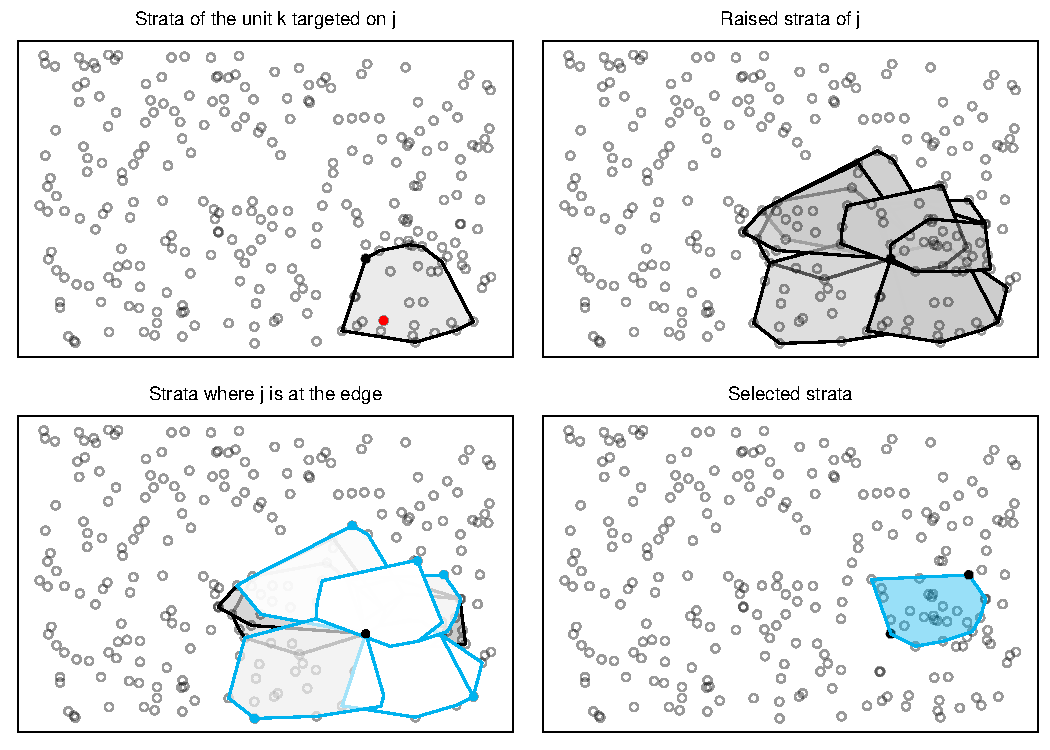
\includegraphics[width=\maxwidth]{figure/image-all_strata-1} \caption[Illustration of the convex hull of the four definition of the different strata]{Illustration of the convex hull of the four definition of the different strata.}\label{fig:all_strata}
\end{figure}


\end{knitrout}









\begin{knitrout}
\definecolor{shadecolor}{rgb}{0.973, 0.973, 0.973}\color{fgcolor}\begin{figure}
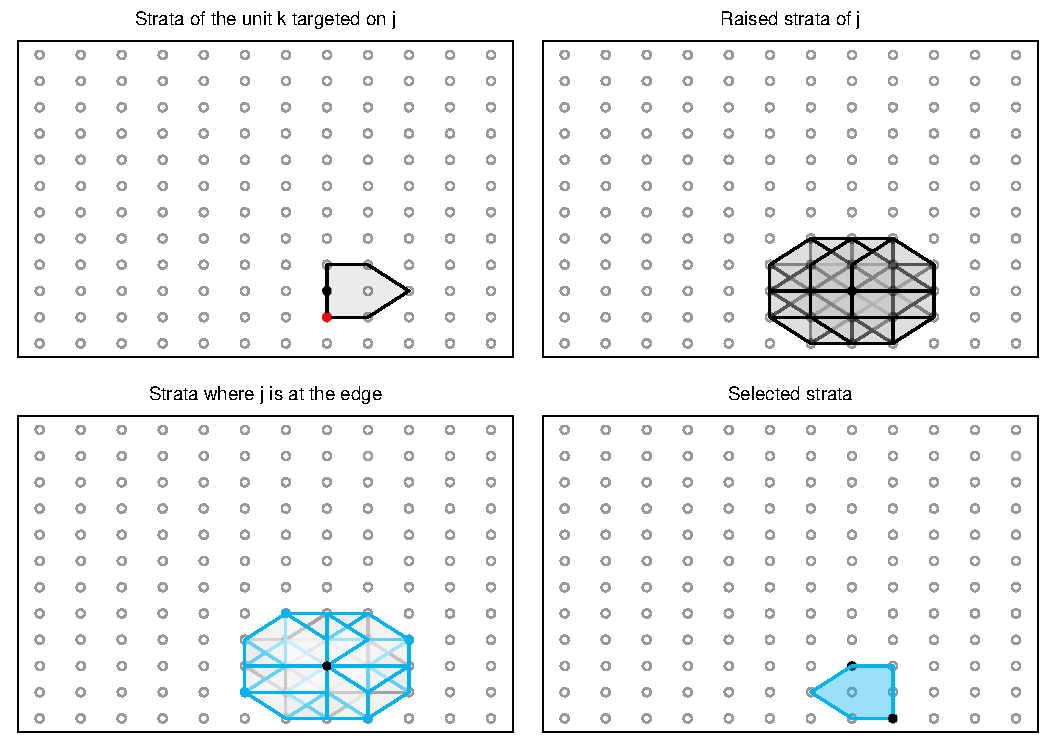
\includegraphics[width=\maxwidth]{figure/image-all_stratagrid-1} \caption[Illustration of the convex hull of the four definition of the different strata]{Illustration of the convex hull of the four definition of the different strata.}\label{fig:all_stratagrid}
\end{figure}


\end{knitrout}

%-----------------------------------------------------------------------------------
%	Tore and shifted distance
%-----------------------------------------------------------------------------------

\subsection{Tore and shifted distance}


%-----------------------------------------------------------------------------------
%	implementation
%-----------------------------------------------------------------------------------

\subsection{Implementation}

We select a starting unit $j$ with respect to the inclusion probabilities $\pig$. We only select a part of the inclusion probability $u$ distributed as a random variable $\mathcal{U}(0,\pi_j)$. Let's define $\pig^\ast$ the vector of inclusion probabilities such that the $\pi_j$ is replaced by $u$. We then looking at the raised strata $R_j$ of the unit $j$  \\


\begin{algorithm}[htb!]
\caption{Algorithm for systematic sampling}\label{algo:sys}
Let $\pig_0  = (\pi_1, \dots, \pi_N) = \pig$ for the initialization step. Select a starting unit $j$ with respect to $\pig$. Generate a random start $u$ distributed as a uniform variable $\mathcal{U}(0,\pi_j)$.
\begin{enumerate}
  \item Define $\pig^\ast = (\pi_1,\dots,\pi_{j-1},u,\pi_{j+1},\dots,\pi_N)$
	\item Compute the raised strata $R_j$ using $\pig^\ast$.
	\item Find the candidate unit that have the minimum distance from the unit $j$ and the modified unit in the strata. Let $i$ be            the index of the modified unit of the selected strata. Let $r_i$ be the quantity not selected in the strata of the unit $i$.
	\item Update $$\pig^\ast =  (\pi_1,\dots, \pi_{i-1},r_i,\pi_{i+1},\dots,\pi_{j-1},\pi_j-u,\pi_{j+1},\dots,\pi_N)$$
	\item Repeat 2. to 4. for the non-zero modified inclusion probabilities until you selected the right number of units.
\end{enumerate}
\end{algorithm}


%-----------------------------------------------------------------------------------
% Spatial Balance
%-----------------------------------------------------------------------------------

\section{Spatial Balance}

%-----------------------------------------------------------------------------------
%	Simulation
%-----------------------------------------------------------------------------------

\section{Simulation}

%-----------------------------------------------------------------------------------
%	Discussion
%-----------------------------------------------------------------------------------

\section{Discussion}


\end{document}
